\section{Description of instrumental DetChar}

I did a whole lot of instrumental DetChar.

\section{Tools and algorithms}

\subsection{Omicron}

We use a sine-Gaussian basis to search for excess power

\subsection{Hveto}

One tool that we have often used in Detector Characterization to look 
for time coincidence between glitches (noise transients) in different 
channels is Hveto (Hierarchical Veto). Glitches in each channel are 
identified by external algorithms that have been tuned to search for 
specific patterns in the time series. Any glitch that is reported in 
the output of an external algorithm is referred to as a trigger. 

Typically, Hveto is used to compare a channel that potentially contains 
gravitational wave signals, denoted $h(t)$, and an auxiliary channel 
that does not have direct astrophysical implications. Hveto counts 
the number of coincident triggers between two time series using a 
user-defined time window centered around each trigger in the auxiliary 
channel. The figure of merit returned by Hveto for each auxiliary channel 
after comparison to $h(t)$ is called \textit{significance}.

Significance answers the following question: how unlikely is it that 
the coincident triggers in these two channels were the result of 
two arbitrary Poisson processes occurring in each channel? 

More specifically, given two arbitrary Poisson processes, how 
unlikely is it that we measure $n$ or more coincident triggers 
given that expected number of coincidences from random chance is $\mu$?

Significance is calculated as (ref Hveto),

\begin{equation}
S = -\log_{10} (\sum\limits_{k = n}^{\infty} P(\mu,k)),
\end{equation}

where $n$ is the number of coincidences found between the two channels 
during the total analysis time and $P(\mu,k)$ is the Poisson probability 
distribution function,
\begin{equation}
P(\mu,k) = \frac{\mu^{k}e^{-\mu}}{k!}.
\end{equation}

Here $\mu$ is the expected number of coincidences between triggers in 
$h(t)$ and the auxiliary channel based solely on chance, which is estimated as,

\begin{equation}
\mu = \frac{N_{h}N_{aux}T_{win}}{T_{tot}},
\end{equation}

where $N_{h}$ and $N_{aux}$ are the number of triggers in $h(t)$ and a 
given auxiliary channel respectively during the total analysis time, 
$T_{tot}$, and $T_{win}$ is the length of the coincidence window used.

A high value of significance indicates that the triggers in the channels 
were very often coincident in time and that there is a very small probability 
that the intersection is a product of random chance. This is a very useful 
measure when we are searching for auxiliary channels that might have some 
noise coupling into our output channel. A significance value of up to 5 is 
often observed in channels with no causal relationship to $h(t)$ (ref Hveto), 
giving us a useful threshold for identifying  effective vetoes.

Another interesting figure of merit used for a given round of Hveto is 
the ratio of $\frac{efficiency}{deadtime}$. Efficiency is defined as the 
percent of triggers vetoed from $h(t)$ during a round of vetoes. Deadtime 
is defined as the percent of total analysis time removed from $h(t)$ during 
a round of vetoes. A ratio of 1 is what we would expect from vetoing time 
at random, indicating no strong time correlation between triggers in the 
two channels. A high value of this ratio, which is ideal, indicates that 
we are vetoing a large number of triggers while maintaining a high percentage 
of our analysis time, indicating that the triggers are often close enough 
in time that we can catch a large number of triggers using a small time window.

When Hveto discovers an auxiliary channel that has a strong correlation 
with $h(t)$, the round winner, it removes all of the time windows surrounding 
auxiliary channel glitches and recalculates the significance of the list of 
auxiliary channels. If a channel's significance has dropped after this removal 
of time, it must have had a large amount of glitches coincident with the 
round winner. The change in significance of each channel is displayed on a 
figure called a `drop-plot`. This is one of the most powerful parts of Hveto
 - the ability to find families of channels that often glitch at the same time.

Ideally, the list of significant channels displayed on the drop-plot will be 
able to localize the issue to a specific subsystem or area of the IFO. 
From there, the issue can be investigated and brought to the attention of 
commissioners for repair or physical inspection. This solution is not possible 
as sometimes the cause of the glitches is unclear, but identifying times of 
poor data quality is still useful.

Using Hveto, we can monitor auxiliary channels to find and remove glitches 
in $h(t)$ that would otherwise pollute a gravitational-wave analysis. Removing 
these glitches serves multiple purposes for the search pipelines. Removing 
high SNR glitches cleans up the background of triggers and allows the search 
pipelines to claim a lower SNR threshold for potential detections. A lower 
SNR threshold implies a larger volume for astrophysical analysis. Removing 
glitches reduces the potential for false alarms in the search pipelines, 
which in turn increases the confidence of eventual detections.


\section{Analog-to-Digital Conversion}

Advanced LIGO interferometers are controlled in real-time using a digital 
control system installed on a series of computers referred to as front end 
computers.  This system overall is referred to as the Front End Control 
(FEC) subsection of the more expansive Control and Data System (CDS).  
In a control loop, the FE computers must be capable of reading in an 
analog signal from the interferometer (position measurements, error signals, 
coil currents, etc), digitally sampling that analog signal, using these now 
digital values in a series of control algorithms, and outputting an analog 
control signal to send back into the interferometer.

The process of digital sampling is handled by an analog-to-digital 
converter (ADC) and the process of analog output is handled by a 
digital-to-analog converter (DAC).  Since these converters are linearly 
mapping a continuous signal onto a discrete range, they are limited by 
their digital bit depth.  For example, a 16 bit ADC is only capable of 
representing $2^{16}$ discrete values, or a range from zero to 65536.  
This range is often centered around zero, giving the ADC the capability 
to handle a range of $\pm32768$.  An incoming analog signal is mapped 
onto this range and converted into a digital signal.

For example, in sampling an analog signal with a range of $\pm100V$, 
10V would be mapped to 32768 digital counts and -10V would be mapped 
to -32768 digital counts with all 
of the intermediate voltage values being linearly mapped to the range. This 
means our digital system would recognize a discrete step size of 
10V/32768 counts $\approx 305 \mu $V/count.

Looking at the system described above, we must be aware of how our system 
is going to react when our analog input signal exceeds the intended maximum 
value of 10V (e.g., an 11V input). The ADC has already assigned its maximum 
digital value to 10V. This is called a digital overflow. In this case the ADC 
will continuously output its maximum value as it has no way to map 11V into 
a discrete value. The same process can occur in a DAC when a digital signal 
is sent out at the maximum allowed digital value. The resulting analog signal 
will be railed at the maximum output value of the DAC, creating a sharp corner 
in the output signal as it flattens out. 

If the digital system is not able to correctly sample and understand an analog 
error signal, it is easy to imagine a scenario where the reponse of the digital 
system and the output control signal are not able to complete the control loop 
as designed. This may cause glitches or misalignments in the interferometer.

We must also consider the fact that many ADCs are calibrated to reflect the 
intended dynamic range of an optic.  If a saturation is occurring, there is 
a good chance that an optic has moved beyond this intended dynamic range, which 
also may cause glitches or misalignments.

The ADCs and DACs are monitored by a series of auxiliary channels, which are 
automatically generated in the front-end system. These auxiliary channels 
monitor each ADC and DAC channel and note when any of the channels has reached 
its digital limit. These channels can be used to generate flags that mark 
ADC and DAC overflows, which can be compared with glitches in $h(t)$ to 
search for glitch mechanisms driven by overflows. These channels can also 
be used to flag any large glitches that cause digital overflows so that they 
can be removed from astrophysical searches. 

Figure \ref{fig:dac-overflow} shows an example of a large glitch that caused 
a digital overflow and was removed from gravitational wave analyses. Figures 
\ref{subfig:strain-dac-overflow} and \ref{subfig:esd-dac-overflow} show a 
large glitch in $h(t)$ and the response of a drive signal that controls 
the motion of ETMY respectively. The signal in \ref{subfig:esd-dac-overflow}, 
which is supposed to be controlling the motion of ETMY, hits its digital 
limit during this glitch. Figure \ref{subfig:etmy-dac-overflow} shows the 
auxiliary channel that monitors this digital overflow incrementing as 
it witnesses the digital overflow. This channel is used to generate 
data quality vetoes that remove times when the ETMY actuation signal has 
hit its digital limit.

\begin{figure}[ht!]%
\centering
\subfloat[]{
  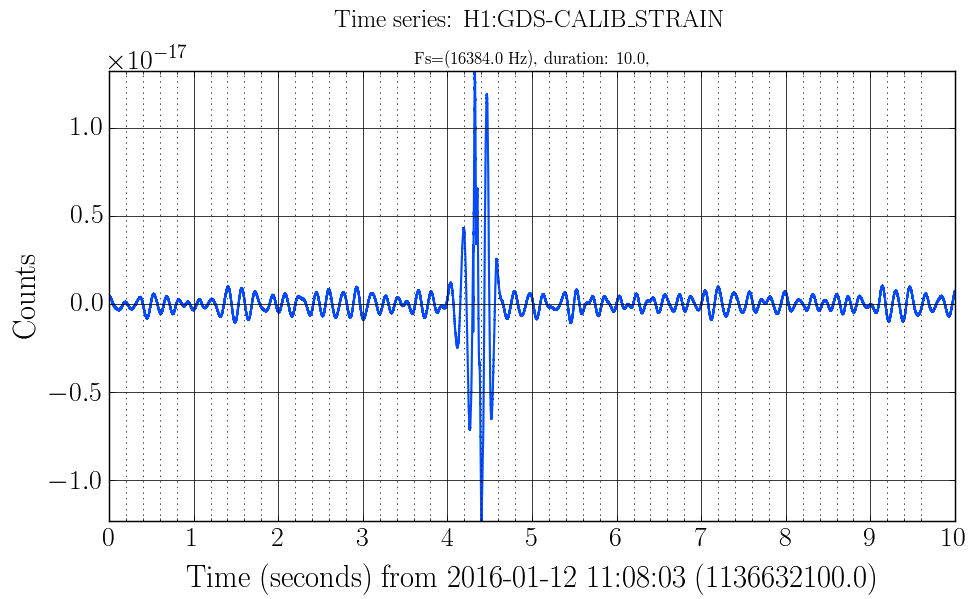
\includegraphics[width=0.495\textwidth]{figures/detchar/strain-dac-overflow}
  \label{subfig:strain-dac-overflow}
  }
\subfloat[]{
  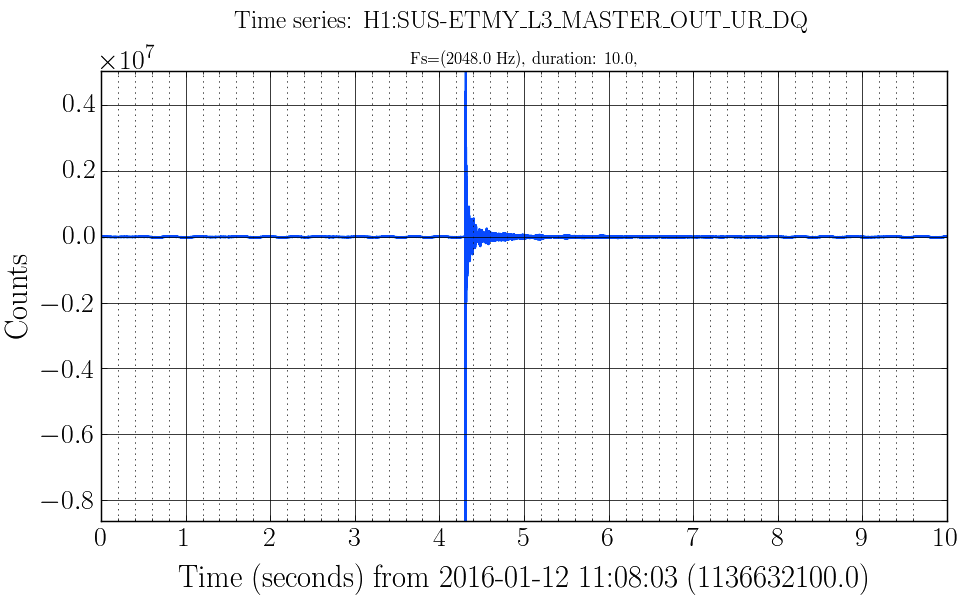
\includegraphics[width=0.495\textwidth]{figures/detchar/esd-dac-overflow}
  \label{subfig:esd-dac-overflow}
  }

\subfloat[]{
  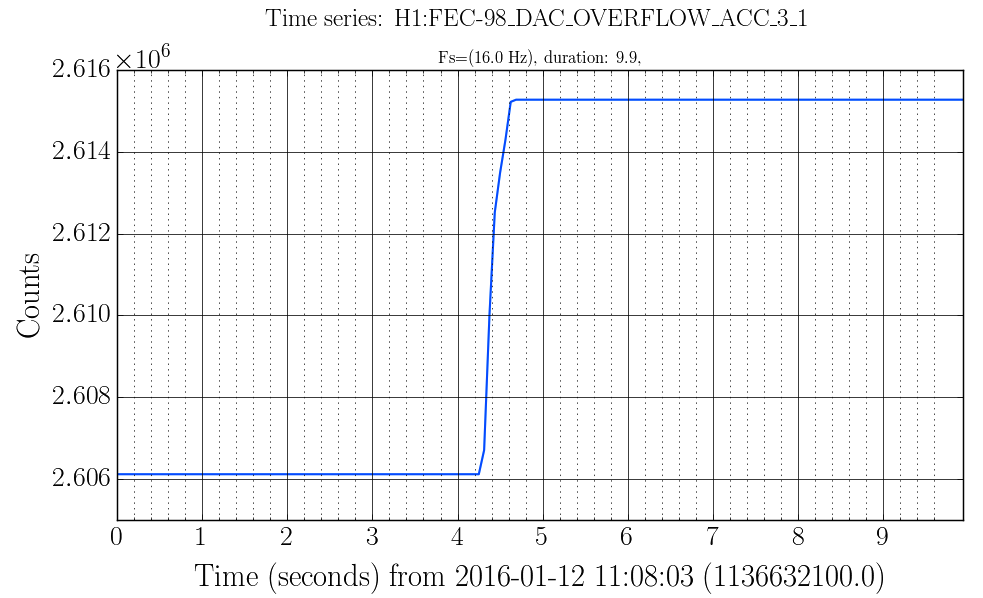
\includegraphics[width=0.495\textwidth]{figures/detchar/etmy-dac-overflow}
  \label{subfig:etmy-dac-overflow}
  }
\caption[ETMY saturation]{Timeseries of an ETMY drive signal saturation in the 
         H1 detector. Figure \ref{subfig:strain-dac-overflow} shows a glitch in 
         the calibrated $h(t)$ channel. Figure \ref{subfig:esd-dac-overflow} shows 
         the response to this glitch in the drive signal used to control the bottom 
         stage of ETMY and actuate on the DARM degree of freedom. This signal hits 
         its digital overflow point at its peak and has no more dynamic range. 
         Figure \ref{subfig:etmy-dac-overflow} shows the front end channel responsible 
         for monitoring digital overflows of this particular ETMY drive signal. 
         Since the witness channel is cumulative, overflows can be identified by 
         flagging any time in which this witness channel is increasing. }
\label{fig:dac-overflow}
\end{figure}

Used this to generate flags for veto definer, ETMY driver and OMC DCPD saturations.

\section{Suspension DAC calibration glitches}

A common glitch mechanism throughout ER6 was due to calibration errors in 
digital-to-analog converters (DACs) responsible for providing analog signals 
to the aLIGO suspensions. The aLIGO suspension subsystem uses 18-bit DACs 
to interact with the optics in the interferometer. These 18-bit DACs are 
created by combining a 16-bit DAC with a 2-bit DAC inside of the same 
electronics box. The 2-bit DAC is responsible for the two highest order 
bits of the output, while the 16-bit DAC is responsible for the 16 lowest 
order bits of the output. If the 16-bit DAC and 2-bit DAC have not had 
their output voltages carefully calibrated, there will be a voltage discontinuity 
at the output of the DAC when engaging the 2 highest order bits. 

Since these DACs use the two's complement 
representation for signed binary numbers, there are two critical points 
where the two highest order bits of the DAC become necessary. The highest 
order bit is used to indicate negative numbers, so an output discontinuity 
is expected when transitioning from a positive number to a negative number, 
that is, crossing through a value of zero.  
The other bit from the 2-bit DAC is used to represent large output values and 
engages when the DAC needs to express a value which is unable to be 
represented by a 16-bit DAC alone. As such, we also 
expect to see discontinuities when the DAC output crosses $\pm2^{16}$. 

The fact that this discontinuity existed in suspension subsystem was 
particularly problematic, as the suspension DACs are used to directly 
actuate on mirror positions and optical cavity lengths. Any time a 
suspension DAC crossed one of these problematic output values, it would 
actuate on the optics with a step function and cause a glitch in the 
optical cavity length. Figure \ref{fig:DAC-glitch} shows an example of 
this issue where the DAC providing actuation signals to the power recycling 
mirror (PRM) is crossing through zero and there are associated glitches 
visible in the length readout of the power recycling cavity.

\begin{figure}[ht!]%
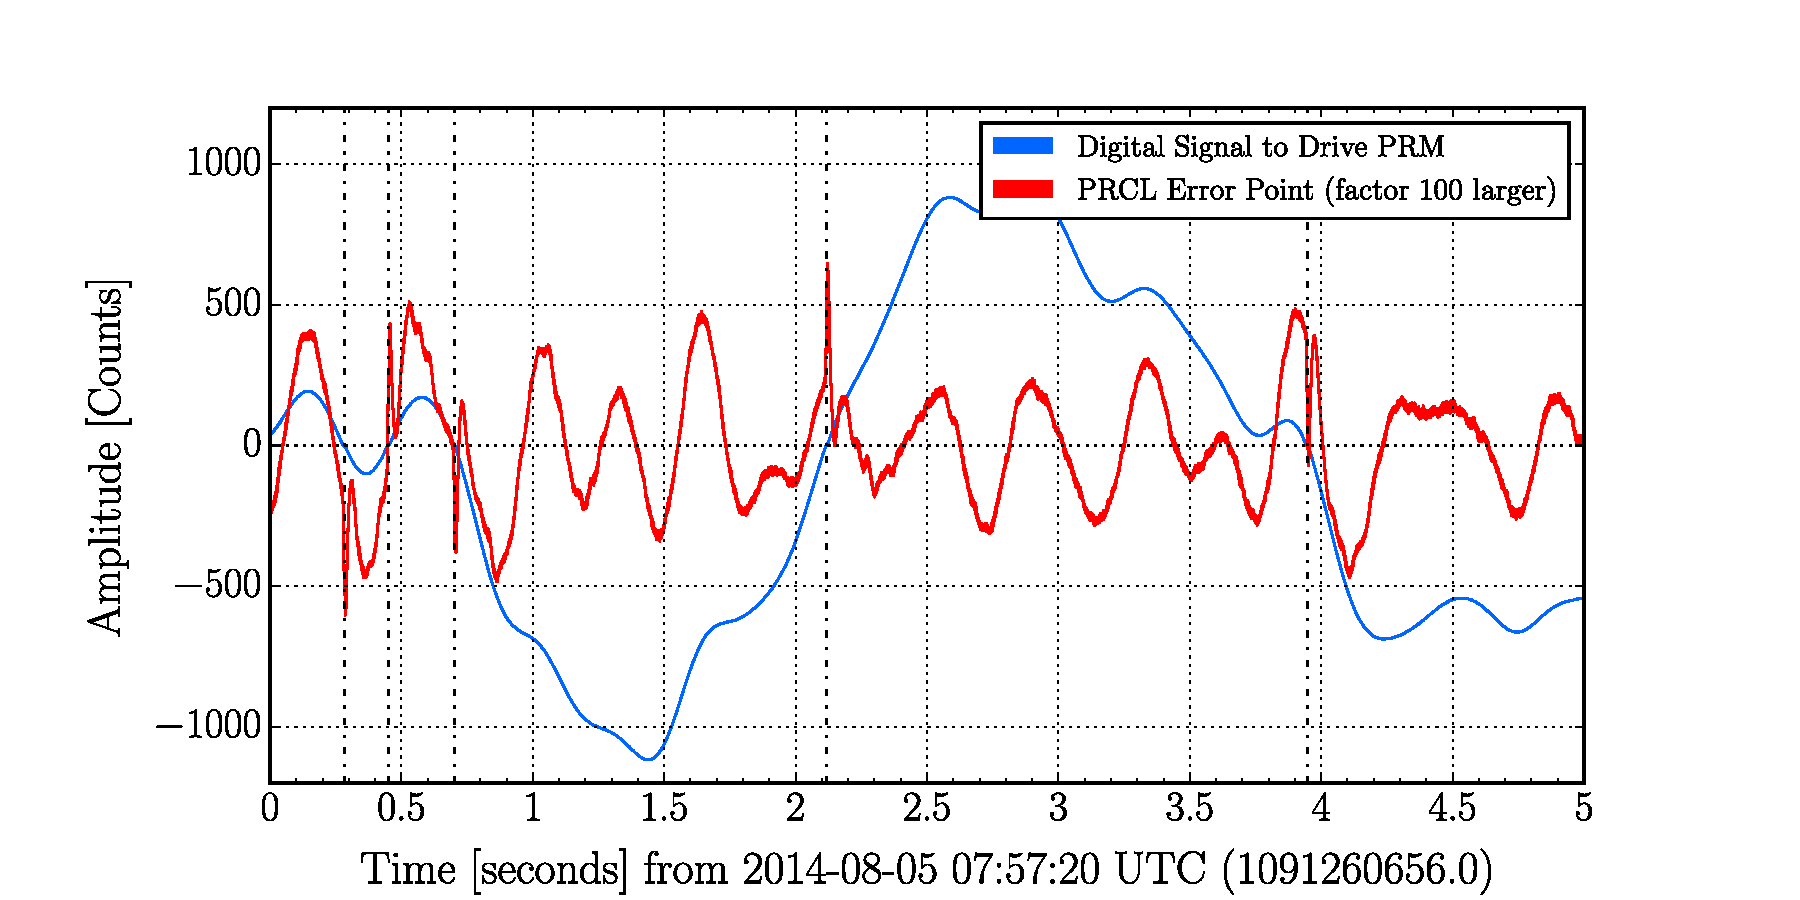
\includegraphics[width=\textwidth]{figures/detchar/PRCL-DAC-glitch}
\caption[DAC glitches in PRCL]{A timeseries plot showing the effects of %
         DAC calibration glitches. The red trace shows the digital drive %
         signal being sent to the digital-to-analog converter. The blue %
         shows the resulting power recycling cavity motion rescaled by a %
         factor of 100. When the drive signal crosses %
         through a value of zero, the output of the DAC experiences a %
         discontinuity, leading to a glitch in the power recycling cavity %
         length.}
\end{figure}\label{fig:DAC-glitch}

The effects of this issue were visible in the $h(t)$ channel during ER6. 
The most problematic culprit was the DAC that applied actuation directly 
to the optics of the ETMs, effectively pushing directly on the DARM degree 
of freedom and causing glitches in $h(t)$. These calibration errors manifested 
themselves as a population of glitches in $h(t)$ recovered by Omicron in the 
20-100 Hz range. This is a very damaging frequency range for CBC searches, 
which hope to accumulate significant SNR in the region from 30-500 Hz.  

\begin{figure}[ht!]%
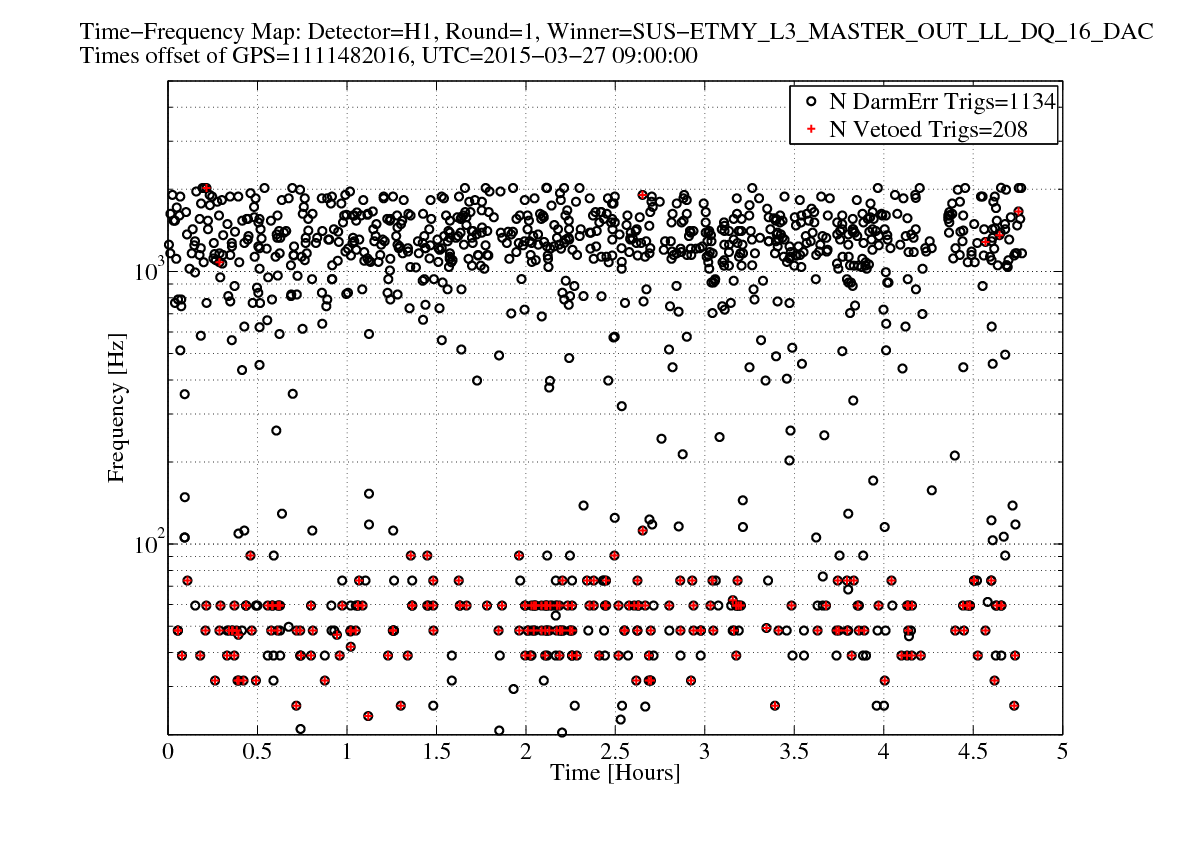
\includegraphics[width=\textwidth]{figures/detchar/vetoed-DAC-glitches}
\caption[Vetoed DARM triggers from DAC calibration]{A time-frequency %
         visualization of Omicron triggers in the H1 $h(t)$ channel. % 
         The black circles indicate glitches in the DARM degree of freedom, %
         each with a central time and central frequency. The red crosses %
         indicate that a given trigger was vetoed by an auxiliary channel %
         trigger which was found to be statistically significant using Hveto. The %
         auxiliary channel triggers in this case indicate that the drive signal %
         on the bottom stage of ETMY has crossed a value of $2^{16}$. The %
         population of glitches between 20 - 100 Hz is highly coincident %
         with these crossings of $2^{16}$, indicating that they are caused %
         by DAC calibration errors on this optic.}
\end{figure}

To fully understand the scope of this problem, the Detector Characterization 
group developed software that searched through the output of all suspension 
DAC digital output signals and marked times when they crossed 0 or $\pm2^{16}$. 
These marked times were converted into trigger files and sent through Hveto 
to look for correlations between crossings of critical values and glitches 
in DARM as identified by Omicron. Through this method, we were able to identify 
which optics were experiencing DAC calibration glitches that had a coupling 
mechanism into DARM.

There were two approaches taken in an effort to mitigate these DAC glitches. The 
first was to introduce offsets into the suspension drive signals so that they 
did not cross through a value of zero. This did solve the problem temporarily, 
but at the cost of a significant portion of the dynamic range of the output 
actuation. The more permanent fix was to run a calibration routine 
that resolved the issue between the 16-bit and 2-bit DACs. This was 
successful, though it had to be run on a weekly basis during site maintenance 
because the calibration tended to drift away from its nominal point after 
2-3 weeks of operation.

During the first observing run, the systematic check of all suspension DAC 
digital output signals was performed again and the resulting triggers were 
sent through Hveto. This study revealed that the calibration process was 
successful; there was no evidence of residual DAC calibration glitches that 
had any noticeable coupling into $h(t)$. The only signal that had any 
significant correlation with glitches in $h(t)$ was not causally sensible. 
Large glitches $h(t)$ were driving the ETMX actuation signal through a value of 
$2^{16}$, which resulted in crossings of $2^{16}$ that were coincident in time 
with glitches in $h(t)$, but weren't representative of calibration errors.

\textcolor{red}{Discuss Hveto results}

\section{RF beatnote whistles}

Two RF oscillators beating against one another creates a kHz beatnote that couples 
into DARM.

\begin{figure}[ht!]%
\centering
\subfloat[]{
  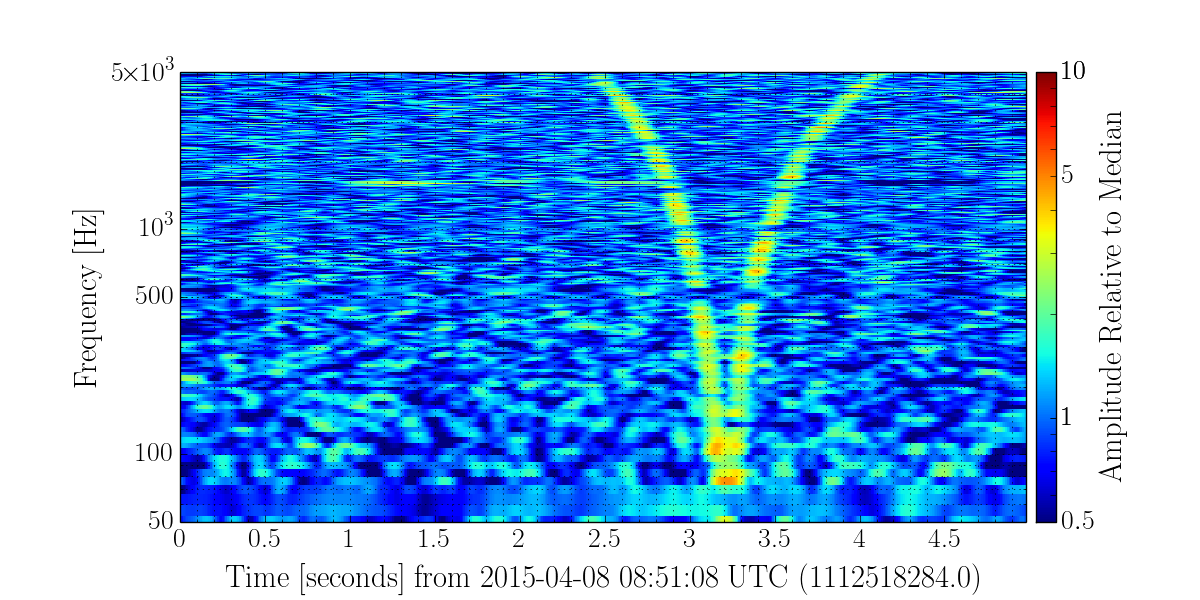
\includegraphics[width=\textwidth]{figures/detchar/Spectrogram_Whistle_LLO}
  \label{subfig:llo-whistle}
  }
  
\subfloat[]{
  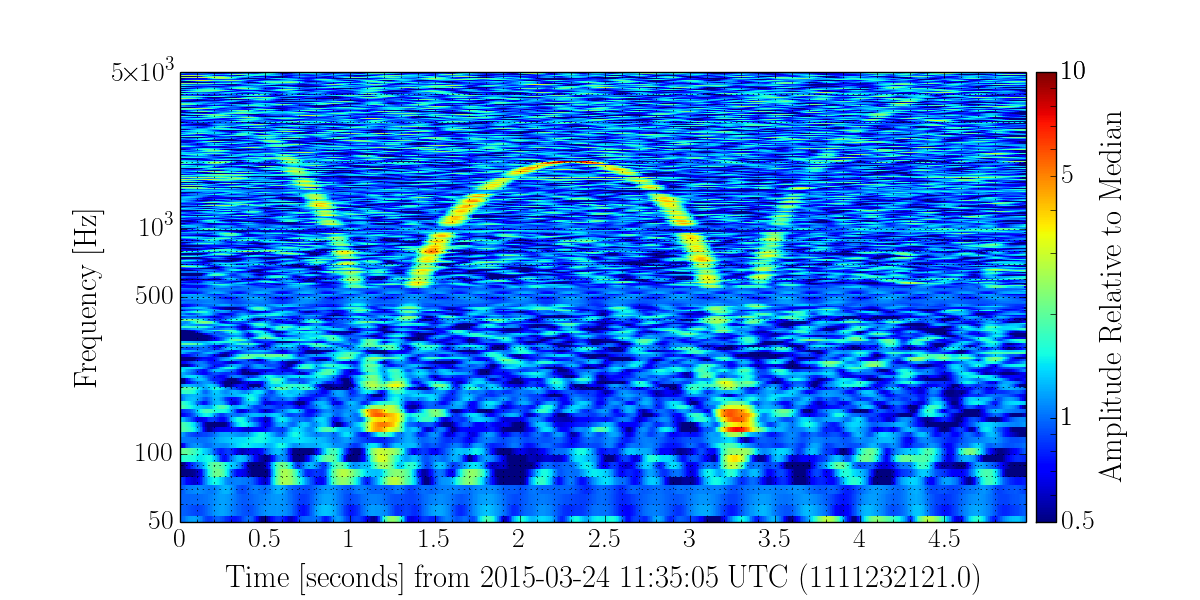
\includegraphics[width=\textwidth]{figures/detchar/Spectrogram_Whistle_LHO}
  \label{subfig:lho-whistle}
  }
\caption[Spectrograms of RF whistles]{Spectrograms of RF whistles at %
         both LLO and LHO. Figure \ref{subfig:llo-whistle} shows a %
         whistle at LLO. Figure \ref{subfig:lho-whistle} shows a whistle %
         at LHO.
         }
\end{figure}\label{fig:whistle-spectrograms}

Hveto shows that a witness channel for RF whistles vetoes approximately 90\% 
of DARM triggers in this time period.

\begin{figure}[ht!]%
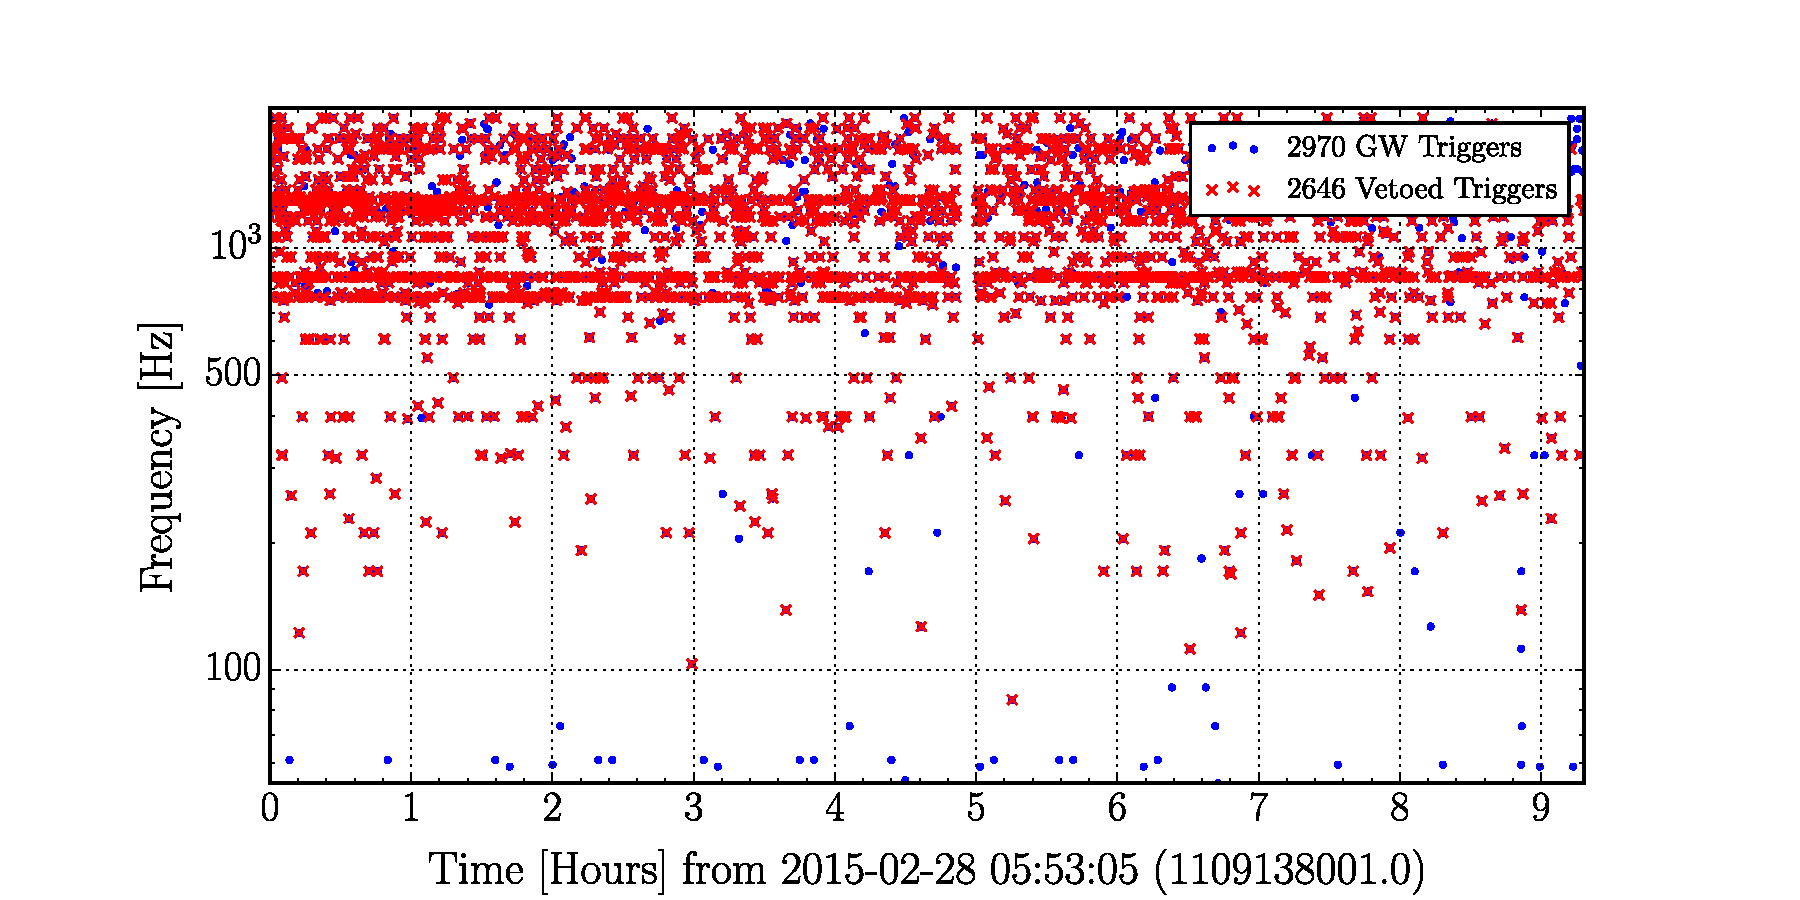
\includegraphics[width=\textwidth]{figures/detchar/Hveto_whistles_time_frequency}
\caption{Black dots are DARM triggers. Red crosses indicate that a trigger was %
         coincident with an RF whistle and vetoed.}
\end{figure}\label{fig:hveto-whistles}

How do we know that the frequency offset worked? Look at a signal that is a proxy 
for the drifting oscillator and histogram all of the Omicron DARM triggers during 
that time. If there's no coupling, the answer should be fairly Gaussian; the 
IFO is just as likely to glitch at any value of the channel. If there are 
channel values that correspond strongly to glitches in DARM, we should see peaks.

\begin{figure}[ht!]%
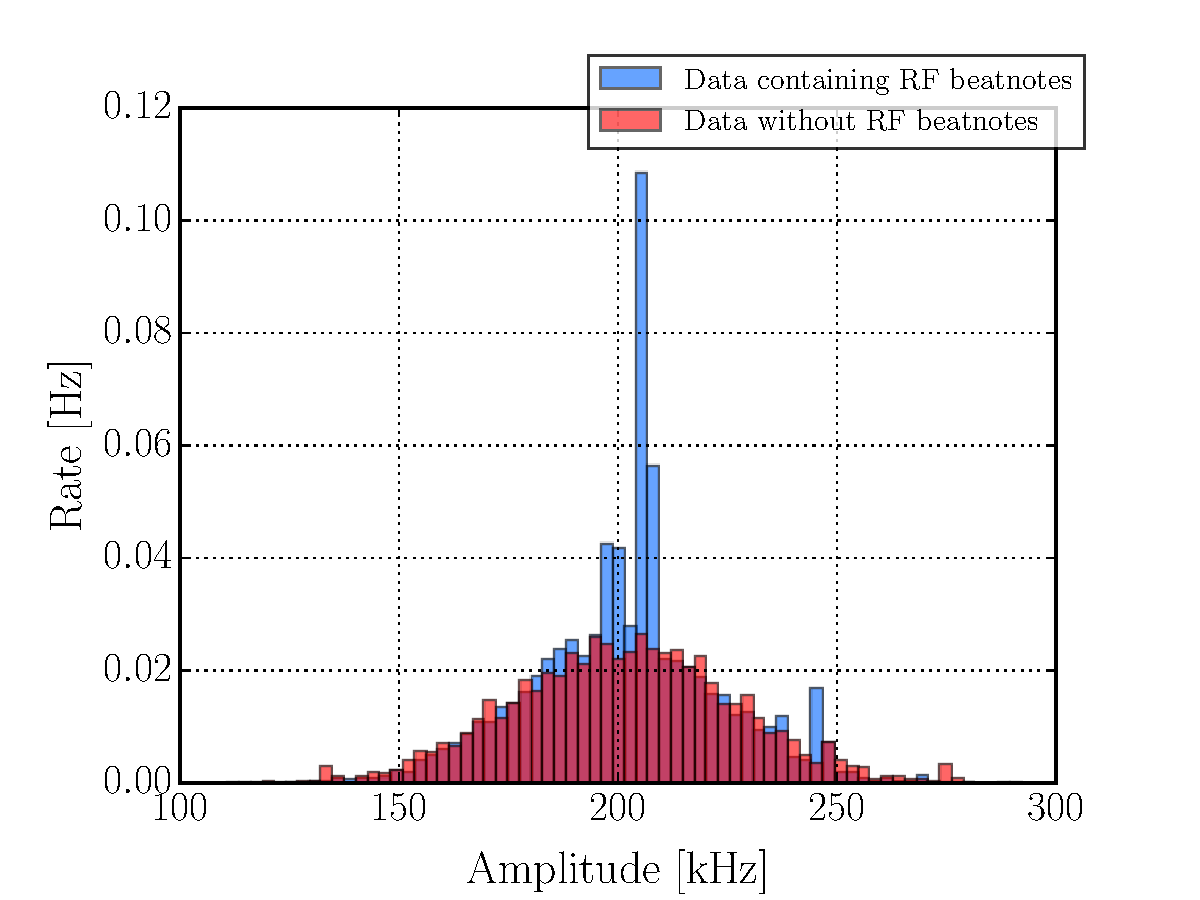
\includegraphics[width=\textwidth]{figures/detchar/Rate_Histogram_Whistles_LLO}
\caption[DARM glitch histograms with and without RF whistles]{Red curve is nice %
         and Gaussian. Blue curve has peaks that indicate problematic frequencies.}
\end{figure}\label{fig:darm-whistle-hist}

\section{Seismic CPS comb}

Oscillators in the capacitive position sensors had drifted apart and caused a 
beatnote and a comb. Audio analysis pointed towards amplitude modulation. 

Fixed by slaving all oscillators to a master.

\section{DC values of auxiliary channels}

No great correlation at the end of the day 

\section{Earthquakes during full lock}

Lots of scattering arches during an earthquake, drove up the noise and biased PSD.
Caused a sarlacc, removing this data was able to repair data on either side.

\section{L1 PMC glitches}


Characterization of noise and analysis after repair

\section{Data quality shifts}
Performed and mentored data quality shifts.



